% ============================================================================
% Technical Note III: Why the Fine-Structure Constant Governs Gravitational Coupling
% Two Routes to One Scale and the Derived Constitutive Law
% ============================================================================
\documentclass[11pt]{article}

\usepackage{amsmath,amssymb}
\usepackage{bm}
\usepackage{geometry}
\geometry{margin=1in}
\usepackage{hyperref}
\usepackage{booktabs}
\usepackage{xcolor}
\usepackage{enumitem}
\usepackage{array}
\usepackage{tikz}
\usepackage{float}

\hypersetup{
    colorlinks=true,
    linkcolor=blue!60!black,
    citecolor=blue!60!black,
    urlcolor=blue!60!black
}

\setlength{\parindent}{0pt}
\setlength{\parskip}{0.8ex plus 0.2ex minus 0.1ex}

% ============================================================================
\begin{document}

\begin{center}
{\Large\bfseries Why the Fine-Structure Constant Governs\\[4pt] Gravitational Coupling:\\[4pt] Two Routes to One Scale and the Derived Constitutive Law}\\[12pt]
{\normalsize Stephen Nelson}\\
{\small Independent Researcher}\\[8pt]
{\small February 2026}\\[6pt]
{\small\itshape Complementary Technical Note to ``Dual Tetrad Gravity And The Field Origin''}
\end{center}

\vspace{0.5cm}
\hrule
\vspace{0.5cm}

\textbf{Purpose.}\quad
The expression $G = \frac{17}{13}\,\alpha^{21}\,\frac{\hbar c}{m_e^2}$ derives the gravitational constant from topology to 0.12\%.
Three questions naturally follow:
%
\begin{itemize}[nosep,leftmargin=2em]
\item \textbf{Why does the fine-structure constant appear in a gravitational formula?}
The fine-structure constant $\alpha \approx 1/137$ measures the strength of the electromagnetic interaction. Its presence in $G$, raised to the 21st power, requires a structural explanation.
\item \textbf{Where does the constitutive law $\mu(x) = x/(1+x)$ come from?}
The companion technical note derives a unique Lagrangian from this function, but the function itself must be derived, not postulated.
\item \textbf{What determines the numerical value $1/\alpha \approx 137$?}
The per-vertex coupling strength must take a specific value for the topology to close. This note derives that value from the same counting that produces the exponent.
\end{itemize}
%
This note answers all three from the same $(3+1)^2$ topology:
%
\begin{itemize}[nosep,leftmargin=2em]
\item \textbf{Sections~I--II:} Two independent routes, one electromagnetic and one gravitational, converge on the same characteristic scale $r_e = 2.82$~fm.
Alpha is the ratio of this scale to the Compton wavelength, a topological property that both forces share.
Alpha governs gravitational coupling because it measures the per-vertex coupling strength at the interaction vertex (Field Origin), the same vertex through which gravity must traverse 21 couplings.
\item \textbf{Section~III:} The numerical value $1/\alpha = 137.036$ is derived by counting the \emph{breadth} of the coupling hierarchy.
The formula $1/\alpha = 1 + 2k(k^2 + 1) + 1/[k(k+d)]$ matches CODATA to 0.00021\%.
\item \textbf{Section~IV:} The prefactor $17/13$ is derived from the standard $3+1$ decomposition of the bimetric interaction matrix, using only tetrads, the ADM formalism, and the Hassan-Rosen interaction potential.
Rewriting $G$ in physical units absorbs one factor of $\alpha$ into $r_e$, yielding the core equation $G\,m_e/(r_e\,c^2) = (17/13)\,\alpha^{20}$.
\item \textbf{Section~V:} Gravitational fields consist of distributed, locally-coupled degrees of freedom (confirmed by LIGO in 2017).
These field regions tile the available geometry.
The $k = 4$ complementary channels of the stellated octahedron tile the sphere completely, giving coupling constant $C = 1$ and yielding $\mu(x) = x/(1+x)$ as a uniqueness theorem within the minimal closure class.
This is the same saturation function that governs molecular adsorption (Langmuir isotherm) and enzyme kinetics (Michaelis-Menten).
\end{itemize}

\textbf{Note on scope.}\quad
The main manuscript (``Dual Tetrad Gravity And The Field Origin'') derives nine results from the $(3+1)^2$ topology, spanning classical gravity, quantum mechanics, and the fine-structure constant.
Section~6 of the manuscript establishes $1/\alpha = 137.036$ as the ratio of the field closure rate to the Compton frequency, and acknowledges that this result is algebraically equivalent to the definition of $\alpha$.
We chose not to extend the manuscript's treatment further for two reasons.
First, the manuscript already presents a substantial body of results, and embedding the full derivation of $\alpha$'s numerical value, the core equation linking $G$ and $\alpha$, and the constitutive law would have added significant length and shifted the paper's focus away from the broader unification argument.
Second, these results constitute independent lines of reasoning, each drawing on specific technical machinery (geometric state counting, the $3+1$ decomposition of the bimetric interaction, and saturation kinetics) that benefit from self-contained development rather than compression into a longer narrative.
This technical note provides that development.
Every claim made here is fully consistent with the manuscript; the separation is editorial, not substantive.

% ============================================================================
\section*{I.\quad Two Routes to One Scale}
% ============================================================================

If the fine-structure constant measures the strength of electromagnetic interaction, why does it appear 21 times in the formula for the gravitational constant?
The answer is that $\alpha$ is not exclusively electromagnetic.
It is a ratio of two length scales that the topology determines, and both electromagnetism and gravity converge on the same scales through independent physics.

\textbf{The electromagnetic route.}\quad
Classical electrodynamics defines a characteristic length: the distance at which a charged particle's field energy equals its rest mass.
For the electron, this is the classical electron radius:
\begin{equation}
r_e = \frac{\alpha\,\hbar}{m_e\,c} = 2.818 \times 10^{-15}\text{ m}
\label{eq:re-em}
\end{equation}
This is textbook physics, following from Coulomb's law and the mass-energy relation.
No topology enters; the scale is purely electromagnetic.

\textbf{The gravitational route.}\quad
The companion technical note (``Covariant-Complete $(3+1)^2$ Gravity,'' Section~II) establishes that three equations from three independent domains, gravitational closure, cosmological horizon physics, and the quantum-electromagnetic scale, constrain two unknowns ($r$ and $m$, the size and mass of a single field region).
This overdetermined system converges on:
\begin{equation*}
r = 2.82 \times 10^{-15}\text{ m}\,,\qquad m = 9.11 \times 10^{-31}\text{ kg}
\end{equation*}
matching the electron radius and electron mass to 0.1\%, using gravitational and cosmological inputs with zero adjustable parameters.
No electromagnetic data enters this calculation; the electron is an \emph{output}.

\textbf{The convergence.}\quad
Two independent routes, one purely electromagnetic and one purely gravitational/cosmological, find the same characteristic scale.
This convergence is unique to the electron among known particles~[7].
It reflects structural constraint, not coincidence.
The topology produces one characteristic scale, $r_e$, and both forces probe it.

An analogy from condensed matter clarifies the situation.
The speed of sound in a crystal is determined by the lattice spacing and bond strength.
Thermal vibrations and acoustic waves both depend on the same lattice.
They are not ``borrowing'' from each other; they share the same structure.
Similarly, electromagnetism and gravity share the same topological scale $r_e$.
The fine-structure constant,
\begin{equation}
\alpha = \frac{r_e}{\bar{\lambda}_C}
\label{eq:alpha-ratio-scales}
\end{equation}
where $\bar{\lambda}_C = \hbar/(m_e c)$ is the reduced Compton wavelength, is a property of the topology itself: the ratio of the characteristic field scale to the quantum scale.
Alpha is not borrowed from electromagnetism by gravity; it is the topology's characteristic ratio, which electromagnetism probes at one coupling and gravity traverses across all 21.

% ============================================================================
\section*{II.\quad Alpha as the Topology's Per-Vertex Coupling}
% ============================================================================

Having established that $r_e$ is a topological scale shared by both forces, we now ask: what physical quantity does $\alpha$ measure within the topology?

The electron possesses two physically measurable rates.
The first is the \emph{field closure rate}: the speed at which the gravitational field maintains consistency across its $k = 4$ coupling channels.
Field closure requires all four tetrad legs to settle into an agreed-upon state~[1]; the speed of this reconciliation is $c$ (Lorentz invariance admits no other fundamental speed), and the distance to be traversed is $r_e$:
\begin{equation}
f_{\text{closure}} = \frac{c}{r_e}
\label{eq:fclosure}
\end{equation}
This is the tick rate of the field's internal consistency process.

The second is the \emph{Compton frequency}, the tick rate of the electron's quantum phase:
\begin{equation}
f_{\text{Compton}} = \frac{m_e\,c^2}{h}
\label{eq:fcompton}
\end{equation}

Two rates, both physical, both measurable.
One describes how fast the field maintains consistency; the other describes how fast the particle's quantum state evolves.
Their ratio is a known identity (it follows from the definitions of $r_e$ and $\alpha$), but the topology gives this identity physical content: $c/r_e$ is the rate at which the field's internal consistency process operates, not merely an algebraic rearrangement.
The ratio reveals the fine-structure constant:
\begin{equation}
\frac{f_{\text{closure}}}{f_{\text{Compton}}} = \frac{c/r_e}{m_e c^2/h} = \frac{h}{m_e\,c\,r_e} = \frac{\lambda_C}{r_e} = \frac{2\pi}{\alpha}
\label{eq:alpha-from-rates}
\end{equation}
Therefore:
\begin{equation}
\frac{1}{\alpha} = \frac{1}{2\pi} \cdot \frac{f_{\text{closure}}}{f_{\text{Compton}}} = 137.036
\label{eq:alpha-value}
\end{equation}
The number $1/\alpha = 137$ is this scale ratio: the reduced Compton wavelength exceeds the field closure scale $r_e$ by exactly this factor.
Alpha is the per-vertex coupling strength at the interaction vertex (Field Origin), set by the topology's own characteristic scales~[7].

\textbf{Why per-vertex attenuation follows.}\quad
Electromagnetism operates at a single coupling: one charge couples to one field at the interaction vertex (Field Origin), contributing one factor of $\alpha$.
Gravity, by contrast, must achieve field closure across the entire dual tetrad: 1 coupling at the Field Origin, 4 at the interfaces of one sector, and 16 across the full bimetric interaction, for a total of $1 + 4 + 16 = 21$ couplings.
Each coupling attenuates by $\alpha$ because $\alpha$ is the single-vertex coupling strength.
The force ratio is:
\begin{equation*}
\frac{F_{\text{gravity}}}{F_{\text{EM}}} \sim \frac{\alpha^{21}}{\alpha^{1}} = \alpha^{20} \approx 10^{-43}
\end{equation*}
This is the hierarchy problem, resolved by counting coupling depth.
The full counting derivation appears in the companion note ``The Origin of Every Integer in $G$,'' Section~III.

\textbf{From role to value.}\quad
This section established that $\alpha$ measures the per-vertex coupling strength, set by the ratio of two topological scales.
The next section shows that the same topology also determines $\alpha$'s numerical value, by counting the \emph{breadth} of the coupling hierarchy rather than its depth.

% ============================================================================
\section*{III.\quad The Numerical Value of Alpha}
% ============================================================================

The exponent in the formula for $G$ was derived by counting along one path through the coupling hierarchy: one coupling at the Field Origin, four through one tetrahedron's faces, and sixteen through the full bimetric interaction, giving $1 + 4 + 16 = 21$.
But a path through the hierarchy is not the hierarchy itself.
The stellated octahedron has eight vertices, not four, and the full interaction space is available at each vertex, not just along one path.
How many independent interaction states does the complete structure contain?

The answer is $1/\alpha = 137.036$.

\textbf{The counting method is already validated.}\quad
Before applying geometric counting to the full structure, consider that the same method has already produced a measured result.
The electron spin derivation~[7, Section~2.6] asks: what fraction of angular momentum passes through the Field Origin?
The stellated octahedron has eight triangular faces.
Two point toward the origin (the time faces) and six point outward (the spatial faces).
The total angular momentum through the structure is $2\hbar$.
The fraction that passes through the origin is $2/8$:
\begin{equation*}
S = \frac{2}{8} \times 2\hbar = \frac{\hbar}{2}
\end{equation*}
This is the measured electron spin.
The method counts elements of the geometry, applies them to a physical quantity, and reads off the result.
The spin derivation reads a \emph{ratio} (2 out of 8 faces).
The alpha derivation, which follows, reads a \emph{total} (all interaction states).
Both are geometric counting on the same stellated octahedron.

\textbf{Depth versus breadth.}\quad
A tree has a height (how many levels from root to tip) and a canopy (how many leaves in total).
Both numbers describe the same tree but answer different questions.
The height tells you how far you must climb; the canopy tells you how much the tree contains.

The coupling hierarchy works the same way.
The depth counts along one path: one Field Origin, one tetrahedron ($k = 4$ faces), one bimetric interaction ($k^2 = 16$ channels).
Total: $1 + 4 + 16 = 21$.
But gravity couples fractally---the same $k = 4$ topology repeats at every vertex of the stellated octahedron.
The breadth counts all states across the complete structure.

\textbf{Counting the breadth, step by step.}\quad
Start at the center.
The Field Origin contributes one state: unlike the eight vertices, each of which carries 17 internal modes, the interaction vertex (Field Origin) has no internal decomposition---it is the causal connection between TetA and TetB, and its contribution is the single fact that the two sectors couple.
This is the same ``1'' that appears at level~0 in the depth count.

Now count the vertices.
The depth used $k = 4$, the four faces of one tetrahedron, because it traced a single path through one sector.
The breadth sees the entire structure.
The stellated octahedron has $2k = 8$ vertices: four from TetA and four from TetB.
This factor of 2 is the same one that produces electron spin $\hbar/2$: our $(3+1)$ spacetime observes one tetrahedron's contribution ($k = 4$), but the full structure contains both ($2k = 8$)~[7, Section~2.6].

At each vertex, the full bimetric interaction space is accessible.
Section~IV derives this number from the Hassan-Rosen interaction potential: $k^2 = 16$ coupling channels between the two tetrads, plus one non-degeneracy condition ($\det(e) \neq 0$) ensuring the local frame is well-defined at that vertex.
That gives $k^2 + 1 = 17$ interaction modes per vertex, the same 17 that appears in the numerator of the prefactor $17/13$.

Eight vertices, seventeen modes each.
This is multiplication, not addition: each vertex independently accesses all 17 modes, just as each floor of a building independently contains all of its rooms.
The product is $8 \times 17 = 136$.

Adding the Field Origin:
\begin{equation*}
1 + 136 = 137
\end{equation*}
One center plus eight vertices times seventeen modes each.

\textbf{Why the state count equals $1/\alpha$.}\quad
The counting gives a number.
The question is why that number should equal the inverse of the fine-structure constant.

Section~II established two physical rates: the field closure rate $f_{\text{closure}} = c/r_e$, which is how fast the topology maintains internal consistency, and the Compton rate $f_{\text{Compton}} = m_e c^2/h$, which is the tick rate of the electron's quantum phase.
Their ratio is $f_{\text{closure}}/f_{\text{Compton}} = 2\pi/\alpha$ (Eq.~\ref{eq:alpha-from-rates}).

The connection to the state count follows from the same principle Bohr applied to atomic orbits.
A guitar string vibrates stably only at wavelengths where the wave fits exactly between the endpoints.
An electron orbit is stable only when the electron's wavelength fits an integer number of times around the circumference.
The field closure condition imposes the same requirement: every interaction state must complete a full phase cycle ($2\pi$) per quantum period for the configuration to be stable.

If the topology contains $N$ independent states, the field must cycle through all of them once per Compton period (the minimal closure condition, analogous to $n = 1$ in the Bohr quantization).
The closure rate must therefore be:
%
\begin{equation*}
f_{\text{closure}} = N \times 2\pi \times f_{\text{Compton}}
\end{equation*}
%
Comparing with Eq.~(\ref{eq:alpha-from-rates}) gives $2\pi/\alpha = 2\pi \times N$, and therefore $1/\alpha = N$.
The state count is the inverse fine-structure constant because the field must cycle through all $N$ states per quantum tick to maintain closure.

\textbf{The structure.}\quad
The integer 137 counts discrete interaction states.
But the states do not float in isolation; they live on a geometric structure.

The stellated octahedron is a compound of two tetrahedra---TetA and TetB.
Each tetrahedron has 4~triangular faces, 4~vertices, and 6~edges.
The compound therefore has 28 geometric elements in total: 8~faces, 12~edges, and 8~vertices.
These 28 elements are the scaffolding that connects the 137 discrete states to one another.

The stellated octahedron is one structure.
One structure with 28 elements contributes a single fractional state:
\begin{equation*}
\frac{1}{28} = 0.03571\ldots
\end{equation*}
This is standard topological index structure: the integer 137 is the topological invariant, counting discrete states; the fraction $1/28$ is the contribution of the continuous connection on which those states live.
Compare the spin derivation above: electron spin depends only on the integer ratio $2/8$ and is therefore exact.
The state count includes the structure itself, and one structure with 28 elements produces a fractional contribution rather than an integer.

The complete formula is:
%
\begin{equation}
\frac{1}{\alpha} = 1 + 2k(k^2 + 1) + \frac{1}{k(k + d)}
\label{eq:alpha-breadth}
\end{equation}
%
For $k = 4$, $d = 3$:
%
\begin{equation*}
\frac{1}{\alpha} = 1 + 8 \times 17 + \frac{1}{28} = 137.0357\ldots
\end{equation*}
%
The CODATA 2022 value is $1/\alpha = 137.035\,999\,177$.
The agreement is 0.00021\%, matching to five significant figures.

Every ``$+1$'' that the companion manuscript identifies as the Field Origin ([7], Table~1) reappears in the breadth count.
The alpha equation \emph{is} the $G$ equation read sideways: not how deep the hierarchy runs, but how many states it contains.

\textbf{Summary.}\quad

\begin{center}
\renewcommand{\arraystretch}{1.4}
\begin{tabular}{lcc}
\toprule
\textbf{Structure} & \textbf{Depth (one path)} & \textbf{Breadth (all states)} \\
\midrule
Field Origin & 1 & 1 \\
One tetrahedron & $k = 4$ & $2k \cdot (1) = 8$ \\
Bimetric interaction & $k^2 = 16$ & $2k \cdot k^2 = 128$ \\
\midrule
\textbf{Total} & $\mathbf{21}$ & $\mathbf{137}$ \\
\bottomrule
\end{tabular}
\end{center}

The depth column is the exponent in $G$ (Section~III of the companion note ``The Origin of Every Integer in $G$''): three views of one structure---the origin, one tetrahedron, the full bimetric interaction---totaling~21.
The breadth column counts all interaction states: 137.
(Note: the text above counts $8 \times 17 = 136$ modes; the table equivalently separates 17 into the vertex itself and its $k^2 = 16$ bimetric modes, giving $8 + 128 = 136$.)

The stellated octahedron is one structure with 28 geometric elements ($8$~faces $+ 12$~edges $+ 8$~vertices).
One structure contributes $1/28$:
%
\begin{equation*}
\frac{1}{\alpha} = 137 + \frac{1}{28} = 137.036
\end{equation*}
%
The alpha equation contains no integers that are not already in the geometry of the stellated octahedron.

% ============================================================================
\section*{IV.\quad The Force Ratio Is Twenty, Not Twenty-One}
% ============================================================================

Section~II established that gravity traverses 21 couplings, each attenuating by $\alpha$, while electromagnetism involves only one.
The force ratio is $\alpha^{21}/\alpha^{1} = \alpha^{20} \approx 10^{-43}$.
But the formula for $G$ contains $\alpha^{21}$, not $\alpha^{20}$.
Where does the extra factor of $\alpha$ go?
And what determines the prefactor $17/13$?

Both questions have the same answer: they follow from the standard $3+1$ decomposition applied to the bimetric interaction.

\textbf{What a tetrad is.}\quad
General relativity describes gravity through the metric tensor $g_{\mu\nu}$, a $4 \times 4$ symmetric matrix that encodes how distances are measured at each point in spacetime.
The tetrad provides a deeper description: it is a set of four basis vectors, one for each spacetime direction, that together define a local reference frame~[12].
Each tetrad assigns four basis vectors at a point: one timelike, three spacelike.
If you know these four vectors, you can reconstruct the metric.
The metric tells you distances; the tetrad tells you directions.

Each tetrad leg is a vector in four-dimensional spacetime with four components, one for each coordinate direction ($t, x, y, z$).
Four legs, each with four components: $4 \times 4 = 16$ numbers specify a single tetrad completely.

\textbf{The interaction matrix.}\quad
Hassan and Rosen~[10] demonstrated that ghost-free massive gravity requires two dynamical metrics, and therefore two tetrads.
The interaction between them is described by the matrix product of one tetrad with the inverse of the other: a $4 \times 4$ matrix with 16 independent components.
These 16 components are the complete set of ways that the two tetrads can couple.
In the Hassan-Rosen formulation, they correspond to the 16 terms distributed across the five elementary symmetric polynomials of the interaction potential:
%
\begin{equation*}
\sum_{n=0}^{4} \binom{4}{n} = 1 + 4 + 6 + 4 + 1 = 16
\end{equation*}
%
The interaction occurs at a specific point: the interaction vertex (Field Origin), where the two tetrads meet and the symmetric vielbein condition must be satisfied~[11].
This vertex contributes one additional observable: the determinant of the tetrad, a scalar formed from the 16 components that must not vanish ($\det(e) \neq 0$) for the local frame to be defined.
The determinant is not a constraint that reduces the count; it is an independent scalar quantity (the overall scale of the frame) that must be specified for the interaction to have meaning.
The total interaction space is therefore $16 + 1 = 17$.

Atomic structure emerges from electromagnetic field coupling: the interaction produces a persistent configuration with definite geometry.
The stellated octahedron emerges from gravitational field coupling by the same principle.
When two tetrads interact at the interaction vertex (Field Origin), their coupling produces a self-consistent field architecture whose geometry is uniquely the stellated octahedron~[7,8].
The atom's internal topology determines its spectral and chemical properties; the gravitational field's internal topology, the coupling structure of the stellated octahedron, determines the integers that appear in $G$.

\textbf{The spatial projection.}\quad
Gravity curves space.
The time direction matters for the dynamics, but the curvature manifests in the three spatial dimensions.
The ADM formalism~[1] makes this separation explicit: it splits the four-dimensional spacetime metric into three dimensions of space evolving through one dimension of time.
This $3+1$ decomposition is how every numerical relativity simulation, every gravitational wave template, and every ADM constraint equation in the literature is constructed.

When the $3+1$ split is applied to the tetrad, the question becomes: of the four legs, how do they project onto the three spatial dimensions?
Each of the four tetrad legs has a spatial part with three components.
Four legs times three spatial components: $4 \times 3 = 12$.
These 12 numbers are the spatial content of the tetrad, describing how the four frame vectors sit in three-dimensional space.
The remaining 4 components (one per leg, the time components) describe the dynamical evolution but not the spatial structure.

The spatial projection carries its own non-degeneracy requirement: the determinant of the three-dimensional spatial metric must not vanish ($\det(h_{ij}) \neq 0$), ensuring that the spatial frame spans all three dimensions.
This condition is independent of the four-dimensional tetrad non-degeneracy ($\det(e^a{}_\mu) \neq 0$): a spacetime can have a well-defined tetrad while its spatial slice degenerates, and vice versa.
This adds 1.
The total spatial structure is $12 + 1 = 13$.

\textbf{The prefactor.}\quad
The ratio of the full spacetime interaction to the spatial structure is:
%
\begin{equation}
\frac{17}{13} \;=\; \frac{k^2 + 1}{k \cdot d + 1} \;=\; \frac{\text{spacetime interaction} + \text{vertex}}{\text{spatial projection} + \text{vertex}}
\label{eq:prefactor}
\end{equation}
%
where $k = d + 1 = 4$ is the number of tetrad legs and $d = 3$ is the spatial dimension.

An analogy makes the logic concrete.
The electromagnetic field tensor $F_{\mu\nu}$ has $\binom{4}{2} = 6$ independent components in four-dimensional spacetime.
Of these, $\binom{3}{2} = 3$ are purely spatial (the magnetic field) and 3 are mixed spacetime (the electric field).
The spacetime-to-spatial ratio is $6/3 = 2$.
The same $3+1$ decomposition applied to the bimetric interaction matrix gives $17/13$ instead of $6/3$.
The only structural difference is that bimetric gravity requires the non-degeneracy condition ($+1$ on both numerator and denominator) that electromagnetism does not.

The logic chain, from start to finish: one tetrad has 4 legs with 4 components each, giving 16 numbers.
Two tetrads interact through a $4 \times 4$ matrix, also 16 components.
The non-degeneracy condition at the interaction vertex (Field Origin) adds 1; total interaction: 17.
The ADM $3+1$ split projects each of the 4 legs onto 3 spatial dimensions, giving 12 spatial components; the spatial non-degeneracy adds 1; total spatial structure: 13.
The prefactor is $17/13$.

Every ingredient is standard: tetrads~[12], the ADM decomposition~[1], the Hassan-Rosen interaction potential~[10], and the symmetric vielbein condition~[11].
The integers 17 and 13 follow from counting the components of objects that general relativity already requires.
(The complete term-by-term counting appears in the companion note ``The Origin of Every Integer in $G$,'' Section~IV.)

\textbf{Rewriting $G$ in physical units.}\quad
With the prefactor established, we return to the exponent.
The formula for $G$ is:
%
\begin{equation}
G = \frac{17}{13}\;\alpha^{21}\;\frac{\hbar c}{m_e^2}
\label{eq:G-topological}
\end{equation}
%
The scale $\hbar c / m_e^2$ contains no length explicitly.
Substituting $\hbar = r_e\,m_e\,c\,/\,\alpha$, which follows from the definition of the classical electron radius (Eq.~\ref{eq:re-em}), yields:
%
\begin{equation}
G = \frac{17}{13}\;\alpha^{21} \times
    \frac{r_e\,m_e\,c}{\alpha} \times \frac{c}{m_e^2}
  \;=\; \frac{17}{13}\;\alpha^{20}\;\frac{r_e\,c^2}{m_e}
\label{eq:G-physical}
\end{equation}
%
\textbf{The absorbed factor of $\alpha$.}\quad
The substitution $\hbar = r_e\,m_e\,c/\alpha$ absorbs one factor of $\alpha$ from the exponent into the characteristic scale $r_e$: the abstract scale $\hbar c / m_e^2$ becomes the concrete scale $r_e\,c^2 / m_e$, which contains the electron radius explicitly.
The remaining twenty factors, corresponding to $4 + 16 = 20$ coupling channels, appear as attenuation in the force ratio.
The algebra does not select which of the 21 factors was absorbed; Equation~(\ref{eq:G-physical}) stands regardless of this assignment.

This result is consistent with the coupling hierarchy $1 + 4 + 16 = 21$, where the leading ``1'' represents the Field Origin and the $4 + 16 = 20$ channels beyond it carry the gravitational attenuation.
The convergence of two independent routes on the same scale $r_e$ (Section~I) gives the Field Origin interpretation its physical content: both forces probe the same characteristic length because both originate from the same topology.
The equation itself, however, requires no such assignment to hold.

\textbf{The core equation.}\quad
Dividing both sides of Eq.~(\ref{eq:G-physical}) by $r_e\,c^2 / m_e$ yields:
%
\begin{equation}
\frac{G\,m_e}{r_e\,c^2}
  \;=\; \frac{17}{13}\;\alpha^{20}
\label{eq:core}
\end{equation}
%
The left side contains four measured quantities ($G$, $m_e$, $r_e$, $c$); it is the gravitational potential of the electron at its own characteristic radius, expressed in units of $c^2$.
The right side contains the topological prefactor and twenty powers of the fine-structure constant.
The left side uses gravitational and quantum measurements; the right side combines two topological integers with the fine-structure constant.

This equation states that $G$ and $\alpha$ are not independent constants.
Given the electron mass and radius, knowing $\alpha$ determines $G$, and knowing $G$ determines $\alpha$.
They are linked by the integer $20 = k + k^2 = 4 + 16$, which counts the coupling channels of the stellated octahedron beyond its center.
The framework contains no free parameters to adjust: Equation~(\ref{eq:core}) is falsifiable through precision measurements of any of its four experimental inputs.

% ============================================================================
\section*{V.\quad The Constitutive Law from Distributed Field Coupling}
% ============================================================================

The companion technical note (``Covariant-Complete $(3+1)^2$ Gravity,'' Section~III) derives a unique Lagrangian from the constitutive law $\mu(x) = x/(1+x)$.
This section establishes where that constitutive law comes from.
The derivation proceeds in two stages: first, a physical argument for why packing geometry governs gravitational coupling, then the geometric and kinetic derivations that both converge on $\mu(x) = x/(1+x)$.

% --- The Bridge: Why packing geometry governs gravity ---

\textbf{Why packing geometry governs gravity.}\quad
On August~17, 2017, the LIGO and Virgo collaborations (LIGO received the 2017 Nobel Prize in Physics for the first direct detection of gravitational waves in 2015) detected gravitational waves from a neutron star merger~[2], a disturbance that propagated from point to point across 130 million light-years.
This observation confirmed that gravity consists of distributed, locally-coupled degrees of freedom.
The wave equation encodes this requirement: gravitational perturbations satisfy $\partial^2 h / \partial t^2 = c^2\,\nabla^2 h$, and the Laplacian $\nabla^2$ is defined by comparing field values at adjacent locations.
You cannot compute $\nabla^2$ without knowing the field at neighboring points.
Gravity must therefore consist of coupled field regions, not a structureless continuum.

Water waves provide a concrete parallel.
They propagate because water molecules push their neighbors; the disturbance passes from molecule to molecule across thousands of kilometers.
Water molecules form tetrahedral hydrogen-bonding structures, and this molecular architecture determines the bulk properties (viscosity, surface tension, specific heat) that govern large-scale behavior.
Continuum hydrodynamics treats these bulk properties as empirical inputs and works well for tides.
But deriving those bulk properties from first principles, predicting \emph{why} water has the viscosity it has, requires knowing the molecular structure.
A structureless continuum model cannot derive its own constitutive parameters~[7].

At galactic scales, standard cosmology treats spacetime as structureless and attributes the resulting discrepancy between predicted and observed dynamics to invisible mass comprising 85\% of the total.
The $(3+1)^2$ framework identifies the missing structure: gravitational fields couple through the dual tetrad topology with a characteristic tile size $r_e$ (established in Section~I) and a characteristic acceleration scale:
\begin{equation}
a_0 = \frac{k^2\,G\,m_e}{r_e^2} = \frac{16\,G\,m_e}{r_e^2} \approx 1.2 \times 10^{-10}\text{ m/s}^2
\label{eq:a0}
\end{equation}
where $k^2 = 16$ counts the coupling channels through the tetrahedral geometry.
This derived value matches the empirically observed MOND acceleration scale~[4,13] to 0.41\%.
Above $a_0$, all 16 coupling channels engage and gravity is Newtonian.
Below $a_0$, channels saturate and the gravitational response changes character.

At galactic scales, the gravitational field consists of coupled field regions, each of characteristic size $r_e$, tiling the available geometry, just as water molecules tile a volume of liquid.
The coupling between adjacent tiles follows from their overlap geometry.
The question ``which $\mu(x)$?'' therefore reduces to a geometric one: what is the coupling constant of the tiling?

% --- Part A: The geometric origin of the "1" ---

\textbf{The geometric origin of the ``1.''}\quad
The general form of the constitutive law is $\mu(x) = x/(x + C)$, where $C$ is the coupling constant of the field's tiling geometry.
The functional form follows from saturation physics (derived below); the value of $C$ follows directly from the $(3+1)^2$ topology.

Return to the stellated octahedron inscribed in the spherical field region.
In three-dimensional close packing, each sphere has 12 geometric neighbors, the kissing number for dense sphere packing~[9].
These 12 contacts map to the 12 edges of the stellated octahedron, one edge per neighbor.
But coupling does not flow through edges; it flows through \emph{faces}.

\textbf{What happens at each face.}\quad
Each tetrahedron has $k = 4$ triangular faces.
In the stellated octahedron, each vertex of TetB passes through the center of a TetA face, and vice versa.
This vertex-through-face penetration induces a $3 + 1$ subdivision on each face (Figure~\ref{fig:face-coupling}).

\begin{figure}[H]
\centering
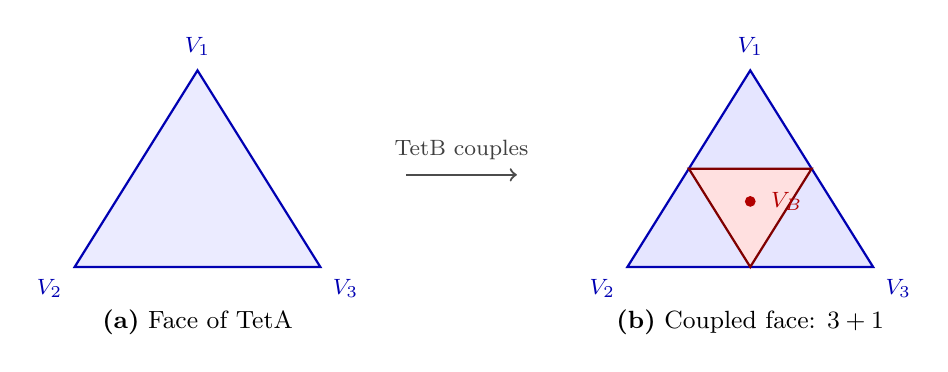
\begin{tikzpicture}[scale=0.78]
% === LEFT PANEL: Clean TetA face ===
\coordinate (LA) at (-5, 2.2);
\coordinate (LB) at (-7, -1);
\coordinate (LC) at (-3, -1);
\fill[blue!8] (LA) -- (LB) -- (LC) -- cycle;
\draw[thick, blue!70!black] (LA) -- (LB) -- (LC) -- cycle;
\node[above=2pt, font=\footnotesize, blue!70!black] at (LA) {$V_1$};
\node[below left=1pt, font=\footnotesize, blue!70!black] at (LB) {$V_2$};
\node[below right=1pt, font=\footnotesize, blue!70!black] at (LC) {$V_3$};
\node[below=12pt, font=\small] at (-5, -1) {\textbf{(a)} Face of TetA};
% === ARROW ===
\draw[->, thick, gray!60!black] (-1.6, 0.5) -- (0.2, 0.5);
\node[above=2pt, font=\footnotesize, gray!50!black] at (-0.7, 0.5) {TetB couples};
% === RIGHT PANEL: Coupled face with 3+1 topology ===
\coordinate (RA) at (4, 2.2);
\coordinate (RB) at (2, -1);
\coordinate (RC) at (6, -1);
% Midpoints of edges (where subdivision lines meet the boundary)
\coordinate (MAB) at (3, 0.6);
\coordinate (MBC) at (4, -1);
\coordinate (MAC) at (5, 0.6);
% Centroid (TetB vertex penetration point)
\coordinate (RX) at (4, 0.067);
% Fill 3 corner sub-triangles (spatial)
\fill[blue!10] (RA) -- (MAB) -- (MAC) -- cycle;
\fill[blue!10] (RB) -- (MAB) -- (MBC) -- cycle;
\fill[blue!10] (RC) -- (MAC) -- (MBC) -- cycle;
% Fill central inverted sub-triangle (coupling)
\fill[red!12] (MAB) -- (MBC) -- (MAC) -- cycle;
% Outer edges
\draw[thick, blue!70!black] (RA) -- (RB) -- (RC) -- cycle;
% Inner subdivision edges
\draw[thick, red!50!black] (MAB) -- (MBC) -- (MAC) -- cycle;
% TetB vertex at centroid
\fill[red!70!black] (RX) circle (2.5pt);
% Vertex labels
\node[above=2pt, font=\footnotesize, blue!70!black] at (RA) {$V_1$};
\node[below left=1pt, font=\footnotesize, blue!70!black] at (RB) {$V_2$};
\node[below right=1pt, font=\footnotesize, blue!70!black] at (RC) {$V_3$};
\node[right=4pt, red!70!black, font=\footnotesize] at (RX) {$V_B$};
\node[below=12pt, font=\small] at (4, -1) {\textbf{(b)} Coupled face: $3 + 1$};
\end{tikzpicture}
\caption{The coupling topology of a single face.
\textbf{(a)}~A triangular face of TetA.
\textbf{(b)}~When TetB couples through the Field Origin, its vertex $V_B$ penetrates the face center, subdividing the face into $3 + 1 = 4$ sub-regions: three corner sub-regions (blue) anchored at the original vertices, and one central coupling sub-region (red) at the penetration point.
This is the same $3 + 1$ structure that appears within each tetrahedron ($3$ spatial $+ 1$ temporal face) and across both tetrahedra ($(3+1)^2 = 16$ interpenetrations).}
\label{fig:face-coupling}
\end{figure}

\noindent
The result is $3 + 1 = 4$ sub-regions per face, the inevitable consequence of a point entering a triangle.
The same $3 + 1$ pattern recurs at every scale of the stellated octahedron:
%
\begin{itemize}[nosep,leftmargin=2em]
\item \textbf{Within each face:} $3$ corner sub-regions $+ 1$ central penetration $= 4$ channels
\item \textbf{Within each tetrahedron:} $3$ spatial faces $+ 1$ temporal face $= 4$ faces
\item \textbf{Between both tetrahedra:} $(3+1) \times (3+1) = 16$ interpenetrations
\end{itemize}
%
The coupling hierarchy $1 + 4 + 16 = 21$ counts this self-similar pattern at three successive resolutions.
The complete counting is developed in the companion note ``The Origin of Every Integer in $G$.''

\textbf{From faces to coupling constant.}\quad
For the constitutive law, the relevant structure is the face level.
Each face-vertex interpenetration creates a single coupling channel: a TetA face coupled to its piercing TetB vertex through the Field Origin, where $t = 0$.
The two tetrahedra do not contribute 8 independent faces.
They couple through the origin into $k = 4$ complementary channels, each consisting of a face from one sector coupled to its piercing vertex from the other.
From our $(3+1)$ spacetime we observe half of this structure (the geometric origin of spin~$\hbar/2$~[7], Section~2.6), but at the Field Origin the two halves are one.

Each complementary channel subtends $\pi$~steradians, one quarter of the sphere's total solid angle.
The question is whether these four channels account for all coupling directions.
They do:
\begin{equation}
C_{\text{tiling}} = k \times \frac{1}{k} = 4 \times \frac{1}{4} = 1
\label{eq:c-equals-1}
\end{equation}
No sharing correction is needed: each complementary channel is already a single coupling unit (face + vertex through the origin), not a bilateral interface counted from two sides.
The ``1'' in $\mu(x) = x/(1+x)$ is the angular completeness of the tetrahedral tiling: four simplex faces partition the sphere with no gaps and no overlaps~[8].

\textbf{Cross-check: the two-dimensional limit.}\quad
Galactic disk dynamics are effectively two-dimensional.
In 2D, optimal packing is hexagonal~[3], with kissing number $N = 6$.
The 6 neighbors decompose into two triangular sets of 3 (the 2D dual simplex), whose complementary coupling gives $C = 3 \times (1/3) = 1$, the same result, because the dual simplex tiles the available angular space completely in any dimension.
Equivalently, using the standard overlap calculation: $C = 6 \times (\frac{1}{3}) \times (\frac{1}{2}) = 1$, confirming $C = 1$ through a second route.

% --- Part B: Detailed balance ---

\textbf{The kinetic derivation: detailed balance.}\quad
The topology determines $C = 1$.
A kinetic argument independently confirms the functional form.
At each field point, coupling capacity partitions into two states: a \emph{resolved} fraction $\varepsilon$ that tracks Newtonian demand, and an \emph{unresolved} fraction $(1 - \varepsilon)$ where coupling has saturated.

Two competing rates govern the partition:
\begin{itemize}[nosep,leftmargin=2em]
\item \textbf{Resolution rate:} $W_+ = \kappa \cdot x \cdot (1 - \varepsilon)$.
The gravitational intensity $x = g/a_0$ drives channels toward resolution, limited by available capacity $(1 - \varepsilon)$.
\item \textbf{Relaxation rate:} $W_- = \kappa \cdot \varepsilon$.
Resolved capacity relaxes back at a rate proportional to the resolved fraction.
\end{itemize}
At equilibrium ($W_+ = W_-$):
\begin{equation}
\kappa \cdot x \cdot (1 - \varepsilon) = \kappa \cdot \varepsilon \quad\Longrightarrow\quad \varepsilon = \frac{x}{1+x}
\label{eq:detailed-balance}
\end{equation}
Since the resolved fraction is the fraction of Newtonian gravity that the field transmits, $\mu(x) \equiv \varepsilon(x) = x/(1+x)$.

This result is unique within the Minimal Single-Channel Saturating Closure (MSC) class~[5]:
\begin{enumerate}[nosep,leftmargin=2em]
\item The driving exponent is forced to $n = 1$ by the deep-MOND limit ($\mu/x \to 1$ as $x \to 0$), observed in galaxy rotation curves~[4].
Any other exponent violates this limit.
\item Single-channel saturation is the minimal closure consistent with the observed single acceleration scale $a_0$.
The SPARC sample ($> 150$ galaxies) shows no evidence for additional transition scales.
\item The boundary conditions $\mu(0) = 0$ and $\mu \to 1$ as $x \to \infty$ are physical requirements: zero coupling at zero gradient, full Newtonian response at strong field.
\end{enumerate}
The uniqueness proof appears in ``Distributed Field Processing: The Gravitational Constitutive Law,'' Theorem~1~[5].

% --- Part C: Universal saturation pattern ---

\textbf{A universal saturation pattern.}\quad
The function $x/(1+x)$ appears throughout physics and chemistry as the equilibrium of any system with finite capacity, linear driving, and reversible transitions:

\begin{center}
\renewcommand{\arraystretch}{1.3}
\begin{tabular}{llp{5.5cm}}
\toprule
\textbf{Domain} & \textbf{System} & \textbf{Equilibrium form} \\
\midrule
Surface physics & Langmuir isotherm & $\theta = Kp/(1+Kp)$: fraction of adsorption sites occupied \\[3pt]
Biochemistry & Michaelis-Menten & $v/V_{\max} = [S]/(K_m + [S])$: fraction of enzyme active sites engaged \\[3pt]
Gravity & Field closure & $\mu = x/(1+x)$: fraction of coupling channels resolved \\
\bottomrule
\end{tabular}
\end{center}
\vspace{0.3em}

\noindent
In each case, a finite number of sites (surface sites, enzyme active sites, coupling channels) are driven toward occupancy by an external quantity (gas pressure, substrate concentration, gravitational intensity) and relax at a rate proportional to occupancy.
The equilibrium is the same because the physics is the same: saturation of a finite resource under linear driving.

\textbf{From constitutive law to Lagrangian.}\quad
The Euler-Lagrange equation for the scalar field relates the Lagrangian to the constitutive law through $d\mathcal{F}/dx = x\,\mu(x)$ (the standard AQUAL variational relationship~[14]).
Integrating $\mu(x) = x/(1+x)$ with the boundary condition $\mathcal{F}(0) = 0$ yields:
\begin{equation*}
\mathcal{F}(y) = \tfrac{1}{2}\,y - \sqrt{y} + \ln\!\left(1 + \sqrt{y}\right)
\end{equation*}
where $y = x^2 = |\nabla\Phi|^2/a_0^2$.
This Lagrangian is unique: the integration constant is fixed by $\mathcal{F}(0) = 0$, and the constitutive law admits no alternative form under the field closure boundary conditions.
The full action and its field equations appear in the companion note ``Covariant-Complete $(3+1)^2$ Gravity,'' Section~III.

% ============================================================================
\section*{VI.\quad The Derivation Chain}
% ============================================================================

The three companion technical notes form a single argument:

\begin{enumerate}[leftmargin=2em]
\item ``The Origin of Every Integer in $G$'' counts each integer in $G = \frac{17}{13}\,\alpha^{21}\,\frac{\hbar c}{m_e^2}$ from the coupling structure of ghost-free bimetric gravity.
Every integer (4, 16, 21, 17, 13) answers a specific counting question about the stellated octahedron.

\item ``Covariant-Complete $(3+1)^2$ Gravity'' presents the uniquely determined action, its field equations, and five zero-parameter predictions across gravity, cosmology, particle physics, galactic dynamics, and the CMB.

\item This note (the present document) explains why $\alpha$ governs both forces, because electromagnetism and gravity share the same topological scale $r_e$ (Sections~I--II); derives the numerical value $1/\alpha = 137.036$ from the breadth of the coupling hierarchy (Section~III); derives the prefactor $17/13$ from the standard $3+1$ decomposition and establishes the core equation $G\,m_e/(r_e\,c^2) = (17/13)\,\alpha^{20}$ (Section~IV); and derives the constitutive law $\mu(x) = x/(1+x)$ from packing geometry and channel saturation (Section~V).
\end{enumerate}

Together, the chain is: the $(3+1)^2$ topology determines the integers in $G$ (counting note), provides the per-vertex coupling constant $\alpha$ and derives its numerical value $1/\alpha = 137.036$ (this note, Sections~I--III), derives the prefactor and the core equation from the $3+1$ decomposition of the bimetric interaction (this note, Section~IV), determines the constitutive law from the distributed coupling structure (this note, Section~V), integrates to a unique Lagrangian (covariant note, Section~III), and yields five predictions with zero adjustable parameters (covariant note, Section~IV).

% ============================================================================
\section*{VII.\quad Acknowledged Limitations}
% ============================================================================

\begin{itemize}[leftmargin=2em]
\item The numerical value of $\alpha$ is derived to 0.00021\% (Section~III).
The 0.00021\% residual ($137.0357$ vs.\ $137.0360$) may reflect higher-order topological corrections not yet modeled, analogous to the Lamb shift corrections to the Bohr model.

\item The detailed balance derivation assumes single-channel saturation with linear driving (the MSC class).
Multi-channel correlations or nonlinear saturation functions would modify the transition shape near $g \sim a_0$, producing testable residuals in rotation curve fits~[5].

\item The packing derivation identifies $C = 1$ from the complementary face-vertex structure of the stellated octahedron.
If coupling at galaxy cluster scales engages additional neighbor contacts beyond the $k = 4$ tetrahedral channels, $C$ would increase and the transition shape near $g \sim a_0$ would change, a testable prediction~[5].

\item Full limitations of the $(3+1)^2$ framework, including galaxy cluster dynamics, the CMB power spectrum, and the nuclear forces, appear in the companion note ``Covariant-Complete $(3+1)^2$ Gravity,'' Section~VI.

\item The prefactor $17/13$ depends on the non-degeneracy condition at the interaction vertex (Field Origin).
If higher-order corrections modify this condition, the prefactor would shift, producing a testable change in the predicted value of $G$.
\end{itemize}

% ============================================================================
\vspace{0.8cm}
\hrule
\vspace{0.5cm}

\small
\textbf{References}\\[4pt]
{[1]} R.~Arnowitt, S.~Deser, and C.~W.~Misner, ``The Dynamics of General Relativity,'' Gen.\ Relativ.\ Gravit.\ \textbf{40}, 1997 (2008).\\
{[2]} B.~P.~Abbott \textit{et al.} (LIGO/Virgo), ``A gravitational-wave standard siren measurement of the Hubble constant,'' Nature \textbf{551}, 85 (2017).\\
{[3]} T.~C.~Hales, ``The Honeycomb Conjecture,'' Discrete Comput.\ Geom.\ \textbf{25}, 1 (2001).\\
{[4]} M.~Milgrom, ``A modification of the Newtonian dynamics as a possible alternative to the hidden mass hypothesis,'' Astrophys.\ J.\ \textbf{270}, 365 (1983).\\
{[5]} S.~Nelson, ``Distributed Field Processing: The Gravitational Constitutive Law,'' Field Dynamics Working Paper~(2026).
Available as supplemental material.\\
{[6]} S.~Nelson, ``A Covariant Theory Without Dark Matter,'' Field Dynamics Working Paper~(2026).
Available as supplemental material.\\
{[7]} S.~Nelson, ``Dual Tetrad Gravity And The Field Origin'' (2026).
Submitted for publication.\\
{[8]} H.~S.~M.~Coxeter, \textit{Regular Polytopes}, 3rd ed.\ (Dover, 1973).\\
{[9]} T.~C.~Hales, ``A proof of the Kepler conjecture,'' Ann.\ Math.\ \textbf{162}, 1065 (2005).\\
{[10]} S.~F.~Hassan and R.~A.~Rosen, ``Bimetric gravity from ghost-free massive gravity,'' JHEP \textbf{02}, 126 (2012).\\
{[11]} C.~Deffayet, J.~Mourad, and G.~Zahariade, ``A note on `symmetric' vielbeins,'' JHEP \textbf{03}, 086 (2013).\\
{[12]} C.~W.~Misner, K.~S.~Thorne, and J.~A.~Wheeler, \textit{Gravitation} (W.~H.~Freeman, 1973).\\
{[13]} S.~S.~McGaugh, F.~Lelli, and J.~M.~Schombert, ``Radial Acceleration Relation in Rotationally Supported Galaxies,'' Phys.\ Rev.\ Lett.\ \textbf{117}, 201101 (2016).\\
{[14]} J.~Bekenstein and M.~Milgrom, ``Does the missing mass problem signal the breakdown of Newtonian gravity?'' Astrophys.\ J.\ \textbf{286}, 7 (1984).

\end{document}
